%% This file is cloned from `sample-sigconf.tex',
\documentclass[sigconf]{acmart}
%% \BibTeX command to typeset BibTeX logo in the docs
\AtBeginDocument{%
  \providecommand\BibTeX{{%
    Bib\TeX}}}
%% Rights management information.  This information is sent to you
%% when you complete the rights form.  These commands have SAMPLE
%% values in them; it is your responsibility as an author to replace
%% the commands and values with those provided to you when you
%% complete the rights form.
\setcopyright{acmlicensed}
\copyrightyear{2024}
\acmYear{2024}
\acmDOI{XXXXXXX.XXXXXXX}

% 29th European Conference on Pattern Languages of Programs
% https://www.europlop.net

%% These commands are for a PROCEEDINGS abstract or paper.
\acmConference[EuroPLoP '24]{29th European Conference on Pattern Languages of Programs}{July 3--7, 2024}{Kloster Irsee, Germany}
%%
%%  Uncomment \acmBooktitle if the title of the proceedings is different
%%  from ``Proceedings of ...''!
%%
%%\acmBooktitle{Woodstock '18: ACM Symposium on Neural Gaze Detection,
%%  June 03--05, 2018, Woodstock, NY}
\acmISBN{978-1-4503-XXXX-X/18/06}
% ============================================================
%\usepackage{a4wide}
\usepackage{xspace}
\usepackage{graphicx}
\graphicspath{{figures/}}
% ============================================================
%% Uncomment the next few lines to get sf url links:
%\usepackage{url}            
%\makeatletter
%\def\url@leostyle{%
%  \@ifundefined{selectfont}{\def\UrlFont{\sf}}{\def\UrlFont{\small\sffamily}}}
%\makeatother
%\urlstyle{leo} % Now actually use the newly defined style.
%% Choose coloured or b/w links:
%\usepackage[pdftex,colorlinks=true,pdfstartview=FitV,
% linkcolor=black,citecolor=black,urlcolor=black]{hyperref}
%\usepackage{hyperref}
\usepackage{needspace}
\newcommand{\needlines}[1]{\Needspace{#1\baselineskip}}
\usepackage{paralist}
% ============================================================
%:Markup macros for proof-reading
\usepackage{ifthen}
\usepackage[normalem]{ulem} % for \sout
\usepackage{xcolor}
\newcommand{\ra}{$\rightarrow$}
\newboolean{showedits}
\setboolean{showedits}{true} % toggle to show or hide edits
%\setboolean{showedits}{false} % toggle to show or hide edits
\ifthenelse{\boolean{showedits}}
{
	\newcommand{\meh}[1]{\textcolor{red}{\uwave{#1}}} % please rephrase
	\newcommand{\ins}[1]{\textcolor{blue}{\uline{#1}}} % please insert
	\newcommand{\del}[1]{\textcolor{red}{\sout{#1}}} % please delete
	\newcommand{\chg}[2]{\textcolor{red}{\sout{#1}}{\ra}\textcolor{blue}{\uline{#2}}} % please change
	\newcommand{\nbe}[3]{
		{\colorbox{#3}{\bfseries\sffamily\scriptsize\textcolor{white}{#1}}}
		{\textcolor{#3}{\sf\small$\blacktriangleright$\textit{#2}$\blacktriangleleft$}}}
}{
	\newcommand{\meh}[1]{#1} % please rephrase
	\newcommand{\ins}[1]{#1} % please insert
	\newcommand{\del}[1]{} % please delete
	\newcommand{\chg}[2]{#2}
	\newcommand{\nbe}[3]{}
}
%
\newcommand\rA[1]{\nbe{Reviewer A}{#1}{cyan}}
\newcommand\rB[1]{\nbe{Reviewer B}{#1}{olive}}
\newcommand\rC[1]{\nbe{Reviewer C}{#1}{magenta}}
\newcommand\ANS[1]{\nbe{Response}{#1}{teal}}

\newcommand{\THE}{\ins{the}\xspace} % "the" missing
\newcommand{\A}{\ins{a}\xspace} % "a" missing
\newcommand{\s}{\ins{s}\xspace} % "s" missing
\newcommand{\COMMA}{\ins{,}\xspace} % "," missing
\newcommand{\THAT}{\chg{which}{that}\xspace} % use "that", not "which"

% ============================================================
%:Box comments/edits
\usepackage[most]{tcolorbox}
\ifthenelse{\boolean{showedits}}
{
  \newtcolorbox{inserted}{%
       title=Inserted text:,
       colframe=blue,colback=blue!5!white,
       breakable,
       leftrule=0mm, 
       bottomrule=0mm,
       rightrule=0mm,
       toprule=0mm,
       arc=0mm, outer arc=0mm,
       oversize
  }
  \newtcolorbox{deleted}{%
       title=Deleted text:,
       colframe=red,colback=red!5!white,
       breakable,
       leftrule=0mm, 
       bottomrule=0mm,
       rightrule=0mm,
       toprule=0mm,
       arc=0mm, outer arc=0mm,
       oversize
  }
  \newtcolorbox{refactored}{%
       % title=Heavily modifed/refactored text:,
       title=Rewritten text:,
       colframe=blue,colback=red!5!white,
       breakable,
       leftrule=0mm, 
       bottomrule=0mm,
       rightrule=0mm,
       toprule=0mm,
       arc=0mm, outer arc=0mm,
       oversize
  }
}{
  \newenvironment{inserted}{}{}
  %\newenvironment{deleted}{ \begin{comment} }{ \end{comment} }
  \let\deleted\comment
  \newenvironment{refactored}{}{} 
}
% ============================================================
%:Put edit comments in a really ugly standout display
%\usepackage{ifthen}
%\usepackage{amssymb} % Avoid error: Command `\Bbbk' already defined.
\newboolean{showcomments}
\setboolean{showcomments}{true}
%\setboolean{showcomments}{false}
\newcommand{\id}[1]{$-$Id: scgPaper.tex 32478 2010-04-29 09:11:32Z oscar $-$}
\newcommand{\yellowbox}[1]{\fcolorbox{gray}{yellow}{\bfseries\sffamily\scriptsize#1}}
\newcommand{\triangles}[1]{{\sf\small$\blacktriangleright$\textit{#1}$\blacktriangleleft$}}
\ifthenelse{\boolean{showcomments}}
%{\newcommand{\nb}[2]{{\yellowbox{#1}\triangles{#2}}}
{\newcommand{\nbc}[3]{
 {\colorbox{#3}{\bfseries\sffamily\scriptsize\textcolor{white}{#1}}}
 {\textcolor{#3}{\sf\small$\blacktriangleright$\textit{#2}$\blacktriangleleft$}}}
 \newcommand{\version}{\emph{\scriptsize\id}}}
{\newcommand{\nbc}[3]{}
 \newcommand{\version}{}}
\newcommand{\nb}[2]{\nbc{#1}{#2}{orange}}
\newcommand{\here}{\yellowbox{$\Rightarrow$ CONTINUE HERE $\Leftarrow$}}
\newcommand\rev[2]{\nb{TODO (rev #1)}{#2}} % reviewer comments
\newcommand\fix[1]{\nb{FIX}{#1}}
\newcommand\todo[1]{\nb{TO DO}{#1}}
\newcommand\on[1]{\nbc{ON}{#1}{olive}} % add more author macros here
% ============================================================
\newboolean{isblinded}
\setboolean{isblinded}{true}
%\setboolean{isblinded}{false}
\ifthenelse{\boolean{isblinded}}
{\newcommand\blind[1]{BLINDED\xspace}}
{\newcommand\blind[1]{#1\xspace}}
% ============================================================
\newcommand{\seclabel}[1]{\label{sec:#1}}
%\newcommand{\secref}[1]{Section~\ref{sec:#1}} <- use \autoref instead!
\newcommand{\figlabel}[1]{\label{fig:#1}}
%\newcommand{\figref}[1]{Figure~\ref{fig:#1}}
\newcommand{\tablabel}[1]{\label{tab:#1}}
%\newcommand{\tabref}[1]{Table~\ref{tab:#1}}
% ============================================================
\newcommand{\ie}{\emph{i.e.},\xspace}
\newcommand{\eg}{\emph{e.g.},\xspace}
\newcommand{\etal}{\emph{et al.}\xspace}
\newcommand{\etc}{\emph{etc.}\xspace}
% ============================================================
\newcommand{\st}[1]{{\tt #1}}
% ============================================================
\begin{document}

%% The "title" command has an optional parameter,
%% allowing the author to define a "short title" to be used in page headers.
\title{Moldable Development Patterns}

\author{Oscar Nierstrasz}
\affiliation{%
  \institution{feenk GmbH}
  \city{Wabern}
  \country{Switzerland}}
\email{oscar.nierstrasz@feenk.com}

\author{Tudor G\^irba}
\affiliation{%
  \institution{feenk GmbH}
  \city{Wabern}
  \country{Switzerland}}
\email{tudor.girba@feenk.com}

\renewcommand{\shortauthors}{G\^irba et al.}

\begin{abstract}
\todo{Rewrite.}
Moldable Development is a way to support decision-making by molding the development tools and environment to your problem, thus making the domain concepts visible, explorable, and explainable.
\end{abstract}

% \keywords{TODO}

%\received{20 February 2007}
%\received[revised]{12 March 2009}
%\received[accepted]{5 June 2009}

%%
%% This command processes the author and affiliation and title
%% information and builds the first part of the formatted document.
\maketitle

% ===== Introduction =========================
\section{Introduction}

Software systems are rich sources of knowledge for both developers and non-technical stakeholders.
But it is difficult to extract that knowledge.
The usual views of software systems are
\begin{inparaenum}[(i)]
\item the source code,
\item the running system.
\end{inparaenum}
But neither of these lends itself well to answering questions about the system.
Software analysis tools can help to some extent, but since every system and every problem is different, it is rare for generic analysis tools to scale to arbitrary systems.

Moldable development is an approach to constructing software systems that are \emph{explainable}.
This is achieved by making it cheap to create dozens, hundreds or even thousands of custom tools to answers questions about a software system, \emph{as these questions arise}.
These custom tools consist of small extensions to the \emph{moldable} tools of the IDE, such as the object inspector, the code browser, the debugger and the notebook.

\begin{figure}[h]
  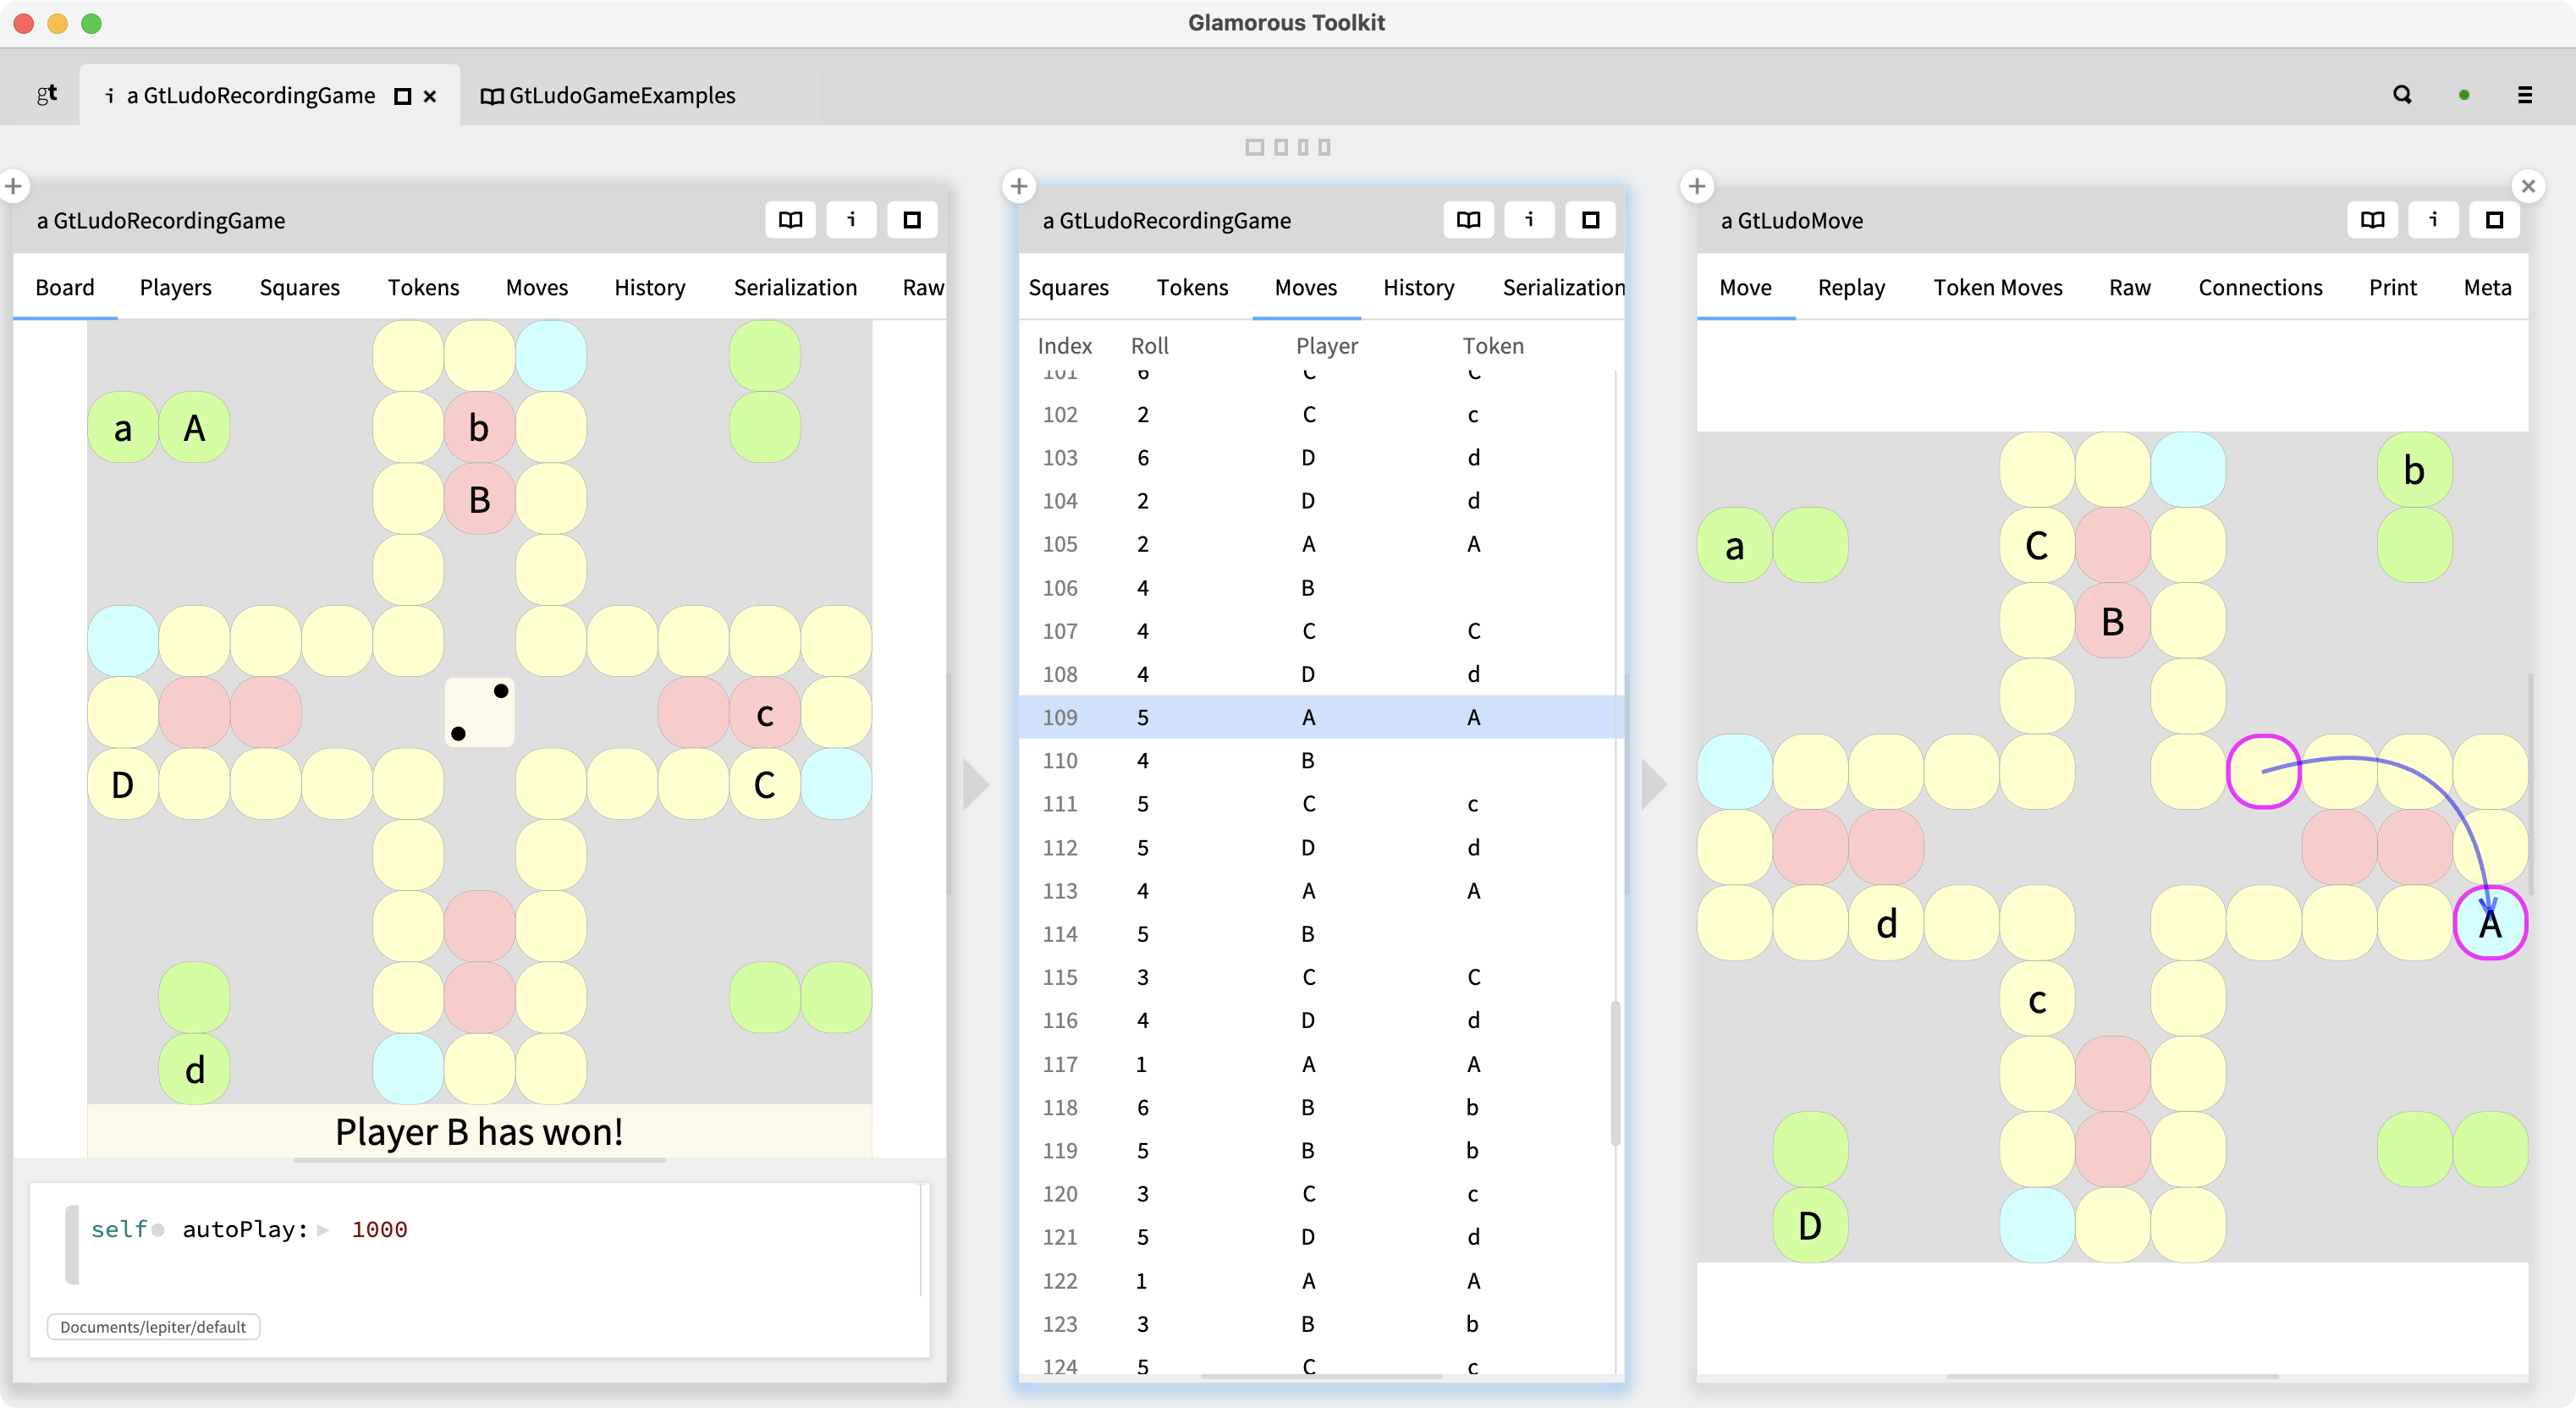
\includegraphics[width=\columnwidth]{custom-views}
  \caption{Custom views of a Ludo game.}
  \label{fig:ludo-views}
\end{figure}

As a simple example, consider the Inspector views of a Ludo game implementation in \autoref{fig:ludo-views}.
With a conventional implementation, we can either try to play the game interactively, or we can stare at the source code.
We can also run the tests, but if these are all green, they do not help us to understand the system.
By applying moldable development, we turn questions we have about the game into custom views.

The figure shows three connected custom Inspector views of a running game.
In the leftmost pane we see the game GUI as the \st{Board} view.
We can also interact programmatically with the game, evaluating ``\st{self autoPlay: 1000}'' in a contextual playground (a kind of REPL).
In the second pane we can explore the moves of  the completed game, and in the third pane we can explore individual moves.
The \st{Move} view visualizes the actual move performed in the context of the current game state at that point in time.
Each of these views is achieved with just a few lines of code, and leads to the Ludo game becoming an explainable system that can be explored in ways that are far richer and more intuitive than by trying to read source code.





\todo{explain Facilitator and Stakeholder}

\todo{introduce map}

\begin{figure}[h]
  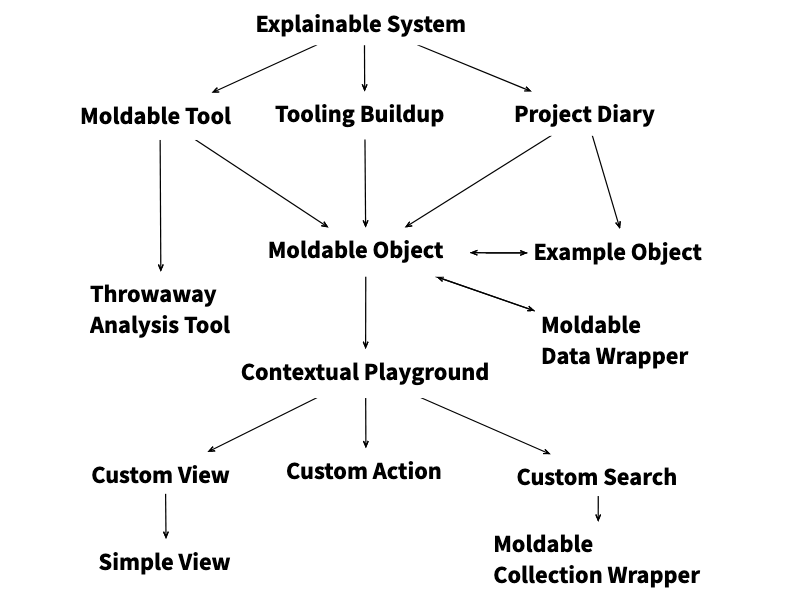
\includegraphics[width=\columnwidth]{map}
  \caption{A map of moldable development patterns.}
  \label{fig:map}
\end{figure}


% ===== Moldable Development Patterns =========================
\section{Moldable Development Patterns}



% ----- PATTERN -------------------------
\subsection{Explainable System}
\subsubsection*{Context}
\subsubsection*{Problem}
\subsubsection*{Forces}
\subsubsection*{Solution}
\subsubsection*{Consequences}



% ----- PATTERN -------------------------
\subsection{Moldable Tool}
\cite{Chis17a}
\subsubsection*{Context}
\subsubsection*{Problem}
\subsubsection*{Forces}
\subsubsection*{Solution}
\subsubsection*{Consequences}



% ----- PATTERN -------------------------
\subsection{Tooling Buildup}
\subsubsection*{Context}
\subsubsection*{Problem}
\subsubsection*{Forces}
\subsubsection*{Solution}
\subsubsection*{Consequences}



% ----- Throwaway Analysis Tool -------------------------
\subsection{Throwaway Analysis Tool}
\subsubsection*{Context}
\subsubsection*{Problem}
\subsubsection*{Forces}
\subsubsection*{Solution}
\subsubsection*{Consequences}


% ----- Project Diary -------------------------
\subsection{Project Diary}
\subsubsection*{Context}
\subsubsection*{Problem}
\subsubsection*{Forces}
\subsubsection*{Solution}
\subsubsection*{Consequences}


% ----- Moldable Object -------------------------
\subsection{Moldable Object}
\subsubsection*{Context}
\subsubsection*{Problem}
\subsubsection*{Forces}
\subsubsection*{Solution}
\subsubsection*{Consequences}

% ----- Example Object -------------------------
\subsection{Example Object}
\subsubsection*{Context}
\subsubsection*{Problem}
\subsubsection*{Forces}
\subsubsection*{Solution}
\subsubsection*{Consequences}

% ----- Viewable Data Wrapper -------------------------
\subsection{Viewable Data Wrapper}
\subsubsection*{Context}
\subsubsection*{Problem}
\subsubsection*{Forces}
\subsubsection*{Solution}
\subsubsection*{Consequences}


% ----- Contextual Playground -------------------------
\subsection{Contextual Playground}
\subsubsection*{Context}
\subsubsection*{Problem}
\subsubsection*{Forces}
\subsubsection*{Solution}
\subsubsection*{Consequences}


% ----- Viewable Entity -------------------------
\subsection{Viewable Entity}
\subsubsection*{Context}
\subsubsection*{Problem}
\subsubsection*{Forces}
\subsubsection*{Solution}
\subsubsection*{Consequences}



% ----- Simple View -------------------------
\subsection{Simple View}
\subsubsection*{Context}
\subsubsection*{Problem}
\subsubsection*{Forces}
\subsubsection*{Solution}
\subsubsection*{Consequences}



% ----- Custom Action -------------------------
\subsection{Custom Action}
\subsubsection*{Context}
\subsubsection*{Problem}
\subsubsection*{Forces}
\subsubsection*{Solution}
\subsubsection*{Consequences}


% ----- PATTERN -------------------------
\subsection{Custom Search}
\subsubsection*{Context}
\subsubsection*{Problem}
\subsubsection*{Forces}
\subsubsection*{Solution}
\subsubsection*{Consequences}


% ----- Collection Wrapper -------------------------
\subsection{Collection Wrapper}
\subsubsection*{Context}
\subsubsection*{Problem}
\subsubsection*{Forces}
\subsubsection*{Solution}
\subsubsection*{Consequences}


%% The next two lines define the bibliography style to be used, and
%% the bibliography file.
\bibliographystyle{ACM-Reference-Format}
\bibliography{moldablePatterns}


\end{document}
\endinput

% ===== TEMPLATES =========================



% ----- PATTERN -------------------------
\subsection{PATTERN}
\subsubsection*{Context}
\subsubsection*{Problem}
\subsubsection*{Forces}
\subsubsection*{Solution}
\subsubsection*{Consequences}


\begin{inparaenum}[(i)]
\item
\item
\end{inparaenum}

